\chapter{Axiomatische Grundlagen}
 \section{Maxwell-Gleichungen}
 \textbf{MGl:=Maxwell-Gleichungen}; Je nach Größen- und \href{https://de.wikipedia.org/wiki/Einheitensystem}{Einheitensystem} sind die Formulierungen von MGl und Materialgleichungen unterschiedlich. Dieses Dokument ist vollständig SI-Konform.
 \subsection{Nomenklatur, Differential- und Integralform}
  \begin{minipage}{0.5\textwidth}
	  \begin{align}
		  \rot\vec{E}+ \frac{\partial \vec{B}}{\partial t} & = \vec{0}\label{ind} \\
		  \div\vec{B}                                      & =0\label{quellf}
	  \end{align}
  \end{minipage}
  \begin{minipage}{0.5\textwidth}
	  \begin{align}
		  \rot\vec{H}-\frac{\partial\vec{D}}{\partial t} & =\vec{J}\label{durchf}        \\
		  \div\vec{D}                                    & =\rho_{\text{V}}\label{gauss}
	  \end{align}
  \end{minipage}
  Während das \textbf{Induktionsgesetz} ($\nearrow$\ref{ind}) und die \textbf{Quellfreiheit
	  des Magnetfeldes} ($\nearrow$\ref{quellf}) \textit{homogene pDGL} sind,
  handelt es sich bei dem \textbf{Durchflutungsgesetz} ($\nearrow$\ref{durchf})
  und dem \textbf{Gaußschen Gesetz} ($\nearrow$\ref{gauss}) um \textit{inhomogene
	  pDGL}. \\Außerdem sind \ref{ind} und \ref{durchf} \textit{vektorielle, zeitabhängige
	  (dynamische) pDGL} und \ref{quellf} und \ref{gauss} \textit{skalare, zeitunabhängige
	  (statische) pDGL}. Die statischen MGl sind \textbf{immer} erfüllt, wenn sie zu \textbf{einem Zeitpunkt} erfüllt sind (eher Nebenbedingungen). \\
  \begin{center} 
	  \begin{tabular}{l c c c l}
		  differentielle Form                                            & $\to$ & Satz   & $\to$ & integrale Form                                                                                                                                                                                 \\
		  \hline
		  $\div \vec{D}= \rho_{\text{V}}$                                & $\to$ & Gauss  & $\to$ & $\oiint\limits_{O(V)}\vec{D}\cdot\dd\vec{A}= \iiint\limits_{V}\rho_{\text{V}}\dd V$                                                                                                            \\
		  $\div \vec{B}= 0$                                              & $\to$ & Gauss  & $\to$ & $\oiint\limits_{O(V)}\vec{B}\cdot \dd\vec{A}= 0$                                                                                                                                               \\
		  $\rot \vec{E}+ \dfrac{\partial \vec{B} }{\partial t}=\vec{0}$  & $\to$ & Stokes & $\to$ & $\oint\limits_{O(A)}\vec{E}\cdot \dd\vec{s}= - \iint\limits_{A}\dfrac{\partial \vec{B} }{\partial t}\cdot\dd\vec{A}$ \\
		  $\rot \vec{H}- \dfrac{\partial \vec{D} }{\partial t}= \vec{J}$ & $\to$ & Stokes & $\to$ & $\oint\limits_{O(A)}\vec{H}\cdot \dd\vec{s}= \iint\limits_{A}\vec{J}\cdot\dd \vec{A} +  \iint\limits_{A}\frac{\partial\vec{D}}{\partial t}\cdot\dd\vec{A}$
	  \end{tabular}\\
	  {\textbf{Überführung von Differential- auf Integralform}}
  \end{center}
  Wenn die Fläche $A$ nicht von der Zeit abhängt, kann man die Differentiation vor das Integral ziehen. Vorgehen bei der Überführung: Bilde das entsprechende Integral über die Differentielle Form und wende den Integralsatz an.
  \subsection{Abgrenzung: Mikroskopische und makroskopische MGl}
  Es ist im allgemeinen sinnvoll, zwischen \textbf{mikroskopischen} und \textbf{makroskopischen} MGl zu unterscheiden. Die mikroskopischen MGl berücksichtigen jeden einzelnen Ladungsträger, \dots. Außerdem können magnetische Eigenschaften bspw. von Permanentmagneten nicht aus diesen abgeleitet werden. Das macht sie unhandlich, weshalb die makroskopischen MGl eingeführt werden, welche die Eigenschaften der Materie in Form von Materialparametern berücksichtigen und mit gemittelten Größen arbeiten ($\nearrow$ mikroskopisch: \ref{mikrosmax}, makroskopisch: \ref{makrmax}).
   \subsection{Begriff: Verschiebungsstromdichte}
  \begin{equation}
  	\vec{J}_D=\frac{\partial\vec{D}}{\partial t}
  \end{equation}
  Die Verschiebungsstromdichte hat zwar die selbe Einheit wie eine elektrische Stromdichte und ruft auch ein Magnetfeld hervor ($\nearrow$\ref{durchf}), ist aber kein Strom im Sinne von sich bewegender Ladung. Mathematisch würde das Nichtvorhandensein dieses Terms zu Widersprüchen führen. Ist $\vec{J}=\rot\vec{H}$, dann ist $\div\vec{J}$ stets 0, was unter anderem im Widerspruch zu \ref{kont} steht. Im folgenden soll phänomenologisch erläutert werden, warum dieser Term im \ref{durchf} notwendig ist. Es wird ein Strom $I$ betrachtet, welcher durch einen langen Draht fließt, in dem sich ein Kondensator befinde (\href{https://commons.wikimedia.org/wiki/File:Displacement_current_in_capacitor.svg}{Bildquelle}):  \begin{center}
  	\resizebox{!}{.6\textwidth}{%% Creator: Inkscape 1.3.2 (1:1.3.2+202311252150+091e20ef0f), www.inkscape.org
%% PDF/EPS/PS + LaTeX output extension by Johan Engelen, 2010
%% Accompanies image file 'Displacement_current_in_capacitor.pdf' (pdf, eps, ps)
%%
%% To include the image in your LaTeX document, write
%%   \input{<filename>.pdf_tex}
%%  instead of
%%   \includegraphics{<filename>.pdf}
%% To scale the image, write
%%   \def\svgwidth{<desired width>}
%%   \input{<filename>.pdf_tex}
%%  instead of
%%   \includegraphics[width=<desired width>]{<filename>.pdf}
%%
%% Images with a different path to the parent latex file can
%% be accessed with the `import' package (which may need to be
%% installed) using
%%   \usepackage{import}
%% in the preamble, and then including the image with
%%   \import{<path to file>}{<filename>.pdf_tex}
%% Alternatively, one can specify
%%   \graphicspath{{<path to file>/}}
%% 
%% For more information, please see info/svg-inkscape on CTAN:
%%   http://tug.ctan.org/tex-archive/info/svg-inkscape
%%
\begingroup%
  \makeatletter%
  \providecommand\color[2][]{%
    \errmessage{(Inkscape) Color is used for the text in Inkscape, but the package 'color.sty' is not loaded}%
    \renewcommand\color[2][]{}%
  }%
  \providecommand\transparent[1]{%
    \errmessage{(Inkscape) Transparency is used (non-zero) for the text in Inkscape, but the package 'transparent.sty' is not loaded}%
    \renewcommand\transparent[1]{}%
  }%
  \providecommand\rotatebox[2]{#2}%
  \newcommand*\fsize{\dimexpr\f@size pt\relax}%
  \newcommand*\lineheight[1]{\fontsize{\fsize}{#1\fsize}\selectfont}%
  \ifx\svgwidth\undefined%
    \setlength{\unitlength}{558.07086182bp}%
    \ifx\svgscale\undefined%
      \relax%
    \else%
      \setlength{\unitlength}{\unitlength * \real{\svgscale}}%
    \fi%
  \else%
    \setlength{\unitlength}{\svgwidth}%
  \fi%
  \global\let\svgwidth\undefined%
  \global\let\svgscale\undefined%
  \makeatother%
  \begin{picture}(1,1.07513228)%
  	\LARGE
    \lineheight{1}%
    \setlength\tabcolsep{0pt}%
    \put(0,0){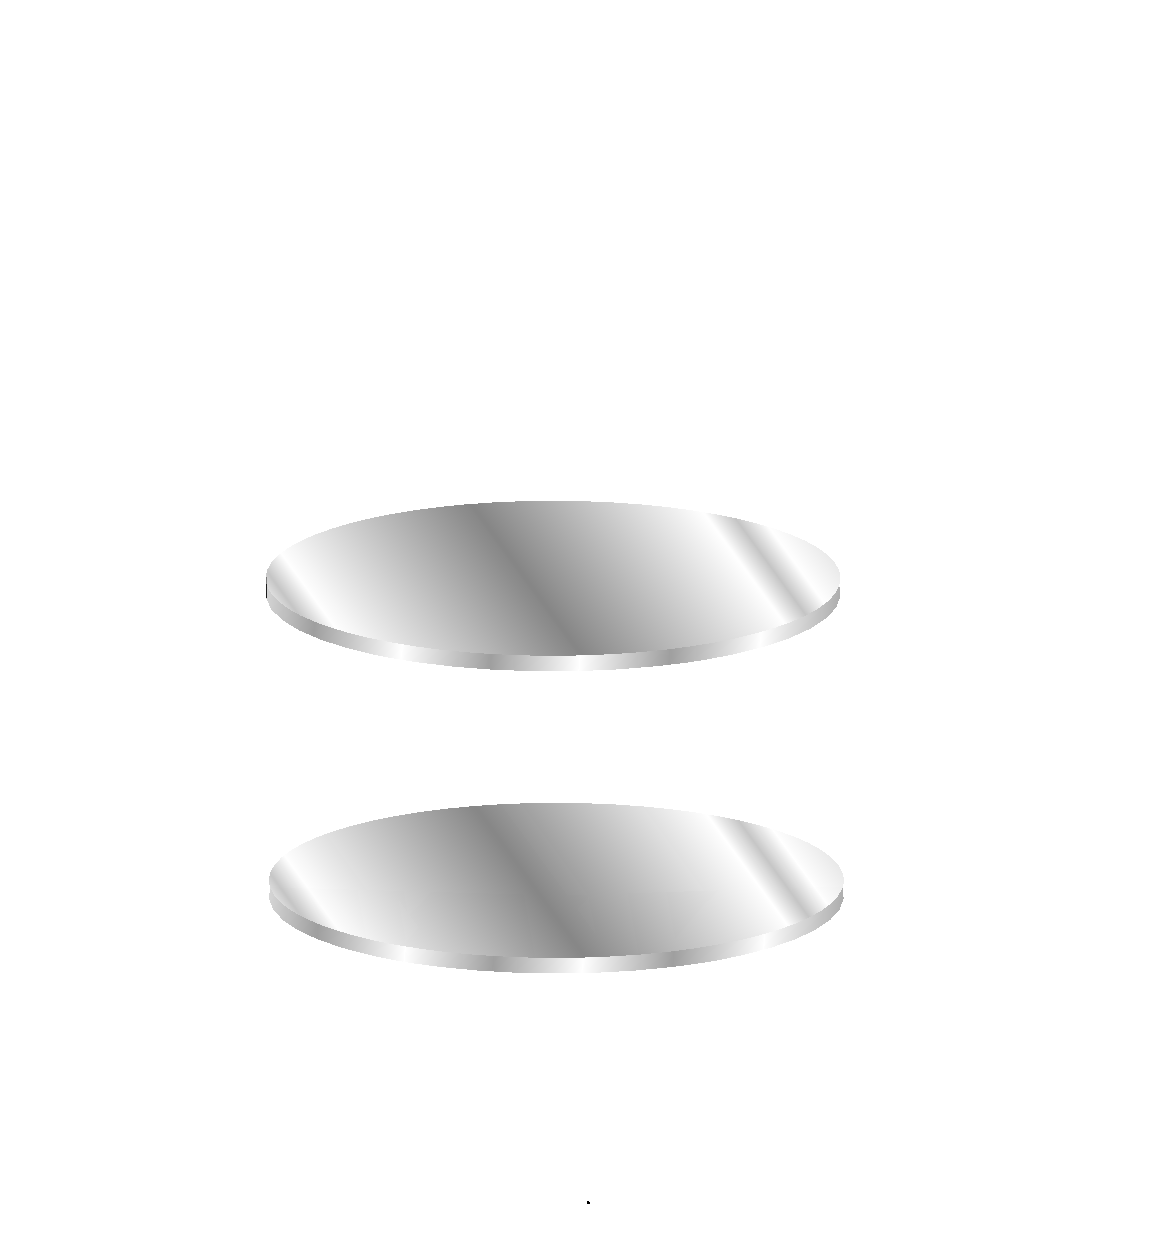
\includegraphics[width=\unitlength,page=1]{res/Displacement_current_in_capacitor.pdf}}%
    \put(0.81736302,0.77152816){\color[rgb]{0.00392157,0,0.02352941}\makebox(0,0)[lt]{\lineheight{0}\smash{\begin{tabular}[t]{l}  \end{tabular}}}}%
    \put(0.80510767,0.77557303){\color[rgb]{0.00392157,0,0.02352941}\makebox(0,0)[lt]{\lineheight{0}\smash{\begin{tabular}[t]{l}$\partial S$\end{tabular}}}}%
    \put(0.71325474,0.38769329){\color[rgb]{0.63921569,0,0}\makebox(0,0)[lt]{\lineheight{0}\smash{\begin{tabular}[t]{l} $\vec{E}$\end{tabular}}}}%
    \put(0.72489797,0.37527524){\color[rgb]{0.63921569,0,0}\makebox(0,0)[lt]{\lineheight{0}\smash{\begin{tabular}[t]{l}  \end{tabular}}}}%
    \put(0,0){\includegraphics[width=\unitlength,page=2]{res/Displacement_current_in_capacitor.pdf}}%
    \put(0.6843464,0.64225882){\color[rgb]{0,0,0}\makebox(0,0)[lt]{\lineheight{0}\smash{\begin{tabular}[t]{l}\textit{ }\end{tabular}}}}%
    \put(0.72235811,0.62596803){\color[rgb]{0,0,0}\makebox(0,0)[lt]{\lineheight{0}\smash{\begin{tabular}[t]{l}\textit{ }\end{tabular}}}}%
    \put(0,0){\includegraphics[width=\unitlength,page=3]{res/Displacement_current_in_capacitor.pdf}}%
    \put(0.36100101,0.9169215){\color[rgb]{0.00392157,0,0.02352941}\makebox(0,0)[lt]{\lineheight{0}\smash{\begin{tabular}[t]{l}$\vec{B}$\end{tabular}}}}%
    \put(0.35215045,0.88599982){\color[rgb]{0.00392157,0,0.02352941}\makebox(0,0)[lt]{\lineheight{0}\smash{\begin{tabular}[t]{l}  \end{tabular}}}}%
    \put(0.34592959,0.9042503){\color[rgb]{0.00392157,0,0.02352941}\makebox(0,0)[lt]{\lineheight{0}\smash{\begin{tabular}[t]{l}  \end{tabular}}}}%
    \put(0.50399451,0.98641512){\color[rgb]{0.00392157,0,0.02352941}\makebox(0,0)[lt]{\lineheight{0}\smash{\begin{tabular}[t]{l} $I$\end{tabular}}}}%
    \put(0.56342076,0.76035686){\color[rgb]{0.00392157,0,0.02352941}\makebox(0,0)[lt]{\lineheight{0}\smash{\begin{tabular}[t]{l}$S_1$\end{tabular}}}}%
    \put(0.70490985,0.6322398){\color[rgb]{0.00392157,0,0.02352941}\makebox(0,0)[lt]{\lineheight{0}\smash{\begin{tabular}[t]{l}$S_2$\end{tabular}}}}%
    \put(0.81445733,0.62002532){\color[rgb]{0.00392157,0,0.02352941}\makebox(0,0)[lt]{\lineheight{0}\smash{\begin{tabular}[t]{l}  \end{tabular}}}}%
    \put(0.49365715,0.07981598){\color[rgb]{0.00392157,0,0.02352941}\makebox(0,0)[lt]{\lineheight{0}\smash{\begin{tabular}[t]{l}$I$\end{tabular}}}}%
  \end{picture}%
\endgroup%
}
  \end{center}
  Nach $\oint\limits_{\partial S}\vec{H}\cdot \dd\vec{s}= I_{S}$ muss das Wegintegral des Magnetfeldes entlang eines beliebigen Weges proportional zu dem Strom sein, der durch eine von diesem Weg aufgespannte Fläche fließt. Bei der türkisen Fläche $S_1$ ist das offensichtlich auch der Fall. Wählt man $S_2$ als Integrationsfläche, muss der Strom exakt der selbe sein, da sich das Magnetfeld auf $\partial S_2=\partial S_1$ durch die Wahl der Fläche nicht ändern darf. Durch den Kondenstator fließt aber kein Strom, was widersprüchlich ist. Hier ändert sich aber der elektrische Fluss. Der Widerspruch kann aufgelöst werden, indem man berücksichtigt, dass auch eine Flussänderung zu einem Magnetfeld führt, was in \ref{durchf} auch passiert.
  \subsection{Komponenten der Stromdichte}
  Eine mögliche Einteilung der Stromdichte ist:
  \begin{equation}
  	\vec{J}=\vec{J}_\mathrm{E}+\vec{J}_\mathrm{L}+\vec{J}_\mathrm{K}
  \end{equation}
  \begin{itemize}
  	\item $\vec{J}_\mathrm{E} = \kappa \vec{E}_\mathrm{E}$ ist die eingeprägte Stromdichte in Bereichen von Urspannung ($\nearrow$\ref{Urspannung}).
  	\item $\vec{J}_\mathrm{L}=\kappa\vec{E}$ ist die Leitungsstromdichte und wird hier meistens betrachtet.
  	\item $\vec{J}_\mathrm{K}$ ist die Konvektionsstromdichte, die z.B. durch Materietransport im Plasma entsteht.
  \end{itemize}
\section{Herleitung wichtiger Gleichungen ($\square$) aus Axiomen und Lemmas}
 \subsection{Poincaré-Lemma} \label{poin}
	   Das Poincaré-Lemma sagt, unter welchen \textbf{Bedingungen} eine Größe
	        als \textbf{Ableitung einer anderen Größe} dargestellt (Potential; nicht
	        Eindeutig $\to$ führt auf den Begriff der Eichung) werden kann. Im Spezialfall 3D-Raum gilt:
	        \begin{enumerate}
		        \item Hat man ein auf einem einfach zusammenhängenden Gebiet wirbelfreies Vektorfeld, dann ist dieses als Gradient eines Potentialfeldes darstellbar:
		              \begin{equation}\label{poin1}
			              \rot\vec{\alpha}=\vec{0}\to \vec{\alpha}= \grad f
		              \end{equation}
		        \item Hat man auf einem konvexen Gebiet ein quellenfreies Vektorfeld, dann ist dieses als Rotation eines Vektorpotentials darstellbar:
		              \begin{equation}\label{poin2}
			              \div \vec{\beta}=0 \to \vec{\beta}= \rot\vec{\alpha}
		              \end{equation}
		        \item Hat man eine skalare Felddichte als Volumenintegrand, dann kann diese als Divergenz eines Vektorfeldes dargestellt werden:
		              \begin{equation}\label{poin3}
			              \gamma \text{ ist ein Volumeintegrand}\to \gamma = \div \vec{\beta}
		              \end{equation}
	        \end{enumerate}
	        

 \subsection{Ladungsdichte und Ladung}
Es gilt, dass die Ladung $Q$ das Volumenintegral über die Ladungsdichte $\rho_{\text{V}}$ ist:
	        \begin{equation}
		        Q = \iiint\limits_{V} \rho_{\text{V}}\dd V \implies \boxed
		        {\div\vec{D} = \rho_\text{V} }
	        \end{equation}
	   Mit dem Poincaré-Lemma ($\rho_{\text{V}}$ ist Integrand eines Volumenintegrals $\to$ sie ist als Divergenz eines Vektorfeldes darstellbar, $\nearrow$\ref{poin3}) folgt unmittelbar das Coulomb-Gauß-Gesetz.\\
	   Ladungen bewegen sich mit der (Material)-Geschwindigkeit $\vec{u}$, damit kann die Stromdichte $\vec{J}$ eingeführt werden:
	        \begin{equation}
		        \vec{J}(\vec{r}) = \rho_{\text{V}}(\vec{r})\vec{u}(\vec{r})
	        \end{equation}
	   Der Strom $I$ ist der Fluss der Stromdichte durch eine 2D-Fläche $S$:
	        \begin{equation}
		        I = \iint\limits_{S} \vec{J}\cdot \dd\vec{A}
	        \end{equation}
 \subsection{Axiom 1: Ladungserhaltung}\label{ladungserhaltung}
 Postulat der Ladungserhaltung: Wenn sich Ladung in einem Volumen ändert, dann geschieht dies nur durch Ladungsstrom durch die Oberfläche des Volumens.
 Betrachtet man die materielle Ableitung (Beobachter bewegt sich mit) $\frac{\mathrm{D}}{\mathrm{D}t}$ und nutzt das Reynolds-Transport-Theorem\footnote{\href{https://de.wikipedia.org/wiki/Transportsatz}{Wikipedia:} Transportsätze beschreiben Regeln für die Zeitableitung von Integralen mit zeitabhängigien Integrationsgrenzen. Das Reynolds-Transport-Theorem ist der Transportsatz für das Volumen.\\\textbf{Aussage:} Gegeben sei ein Kontrollvolumen $V$ mit Volumenelement $\mathrm{d}V$ und Oberfläche $a$ mit nach außen gerichtetem, vektoriellem Oberflächenelement $\mathrm{d}\vec{a}$. Dann lautet die Zeitableitung des Volumenintegrals einer vom Ort $\vec x$ und der Zeit $t$ abhängigen Feldgröße $f(\vec{x},t)$ über das Kontrollvolumen ($\vec{v}$ ist die Geschwindigkeit des Beobachters und des Kontrollvolumens $\to$ Beobachter bewegt sich mit): $\frac{\mathrm{D}}{\mathrm{D}t}\int_V f\,\mathrm{d}V	=\int_V\frac{\partial f}{\partial t}\,\mathrm{d}V
 	+\int_a f\vec{v}\cdot\,\mathrm{d}\vec{a}
 	$ (skalar). $\frac{\mathrm{D}}{\mathrm{D}t}$ ist die Ableitung des Feldes entlang der Bahn des Ladungsteilchens. Die vom Ladungsteilchen auf seiner Bahn wahrgenommene Änderung setzt sich zusammen aus zwei Komponenten: Die Änderung aufgrund verschiedener Feldstärken an den durchlaufenen Orten und einer eventuellen Zeitabhängigkeit des Feldes: $\frac{\text{D}\Phi(\vec{x},t)}{\text{D}t}:=\underbrace{\frac{\partial\Phi}{\partial t}}_\text{zeitlich}+\underbrace{(\vec{v}\cdot\vec{\nabla})\Phi}_\text{durch Bewegung}$.} (*) folgt:
	        \begin{equation}
		        \begin{split}
			        \frac{\mathrm{D} Q}{\mathrm{D} t}&= \frac{\mathrm{D}}{\mathrm{D} t}\left
			        [ \int\limits_{V(t)}\rho_{\text{V}}\dd V \right] \stackrel{!}{=}0\\&\stackrel{*}{=}
			        \int\limits_{V(t)}\frac{\partial \rho_{\text{V}}}{\partial t}\dd V + \oint
			        \limits_{O(V)(t)}\rho_{\text{V}}\vec{u}\cdot \dd\vec{A}\qquad \to \frac{\partial
				        Q}{\partial t}+ \oiint\limits_{O(V)}\vec{J}\cdot d\vec{A}= 0\\\text{Gauss}\to &\stackrel{}{=}
			        \int\limits_{V(t)}\left(\frac{\partial \rho_{\text{V}}}{\partial t}+ \div
			        \left(\rho_{\text{V}}\vec{u}\right) \right) \dd V \\&= \int\limits_{V(t)}
			        \left(\frac{\partial \rho_{\text{V}}}{\partial t}+ \div \vec{J}\right)
			        \dd V \xrightarrow{\textbf{Kontinuitätsgleichung}}\boxed{\frac{\partial \rho_{\text{V}}}{\partial
				        t}+ \div \vec{J}= 0} \\&= \int\limits_{V(t)}\div \left( \frac{\partial
				        \vec{D}}{\partial t}+ \vec{J}\right) \dd V
		        \end{split}
	        \end{equation}

	   Damit dies für beliebige (zeitlich veränderliche) Volumina gelten kann,
	        folgt:
	        \begin{equation}
		        \div \left( \frac{\partial \vec{D}}{\partial t}+ \vec{J}\right) = 0
	        \end{equation}

	   Aus Pointcaré ($\nearrow$\ref{poin2}):
	        \begin{equation}
		        \begin{split}
			        \div \left( \frac{\partial \vec{D}}{\partial t}+ \vec{J}\right) = 0 \to
			        \frac{\partial \vec{D}}{\partial t}+ \vec{J}= \rot\vec{H}&\\ \Aboxed{\rot\vec{H}
			        &- \frac{\partial \vec{D}}{\partial t}= \vec{J}}
		        \end{split}
	        \end{equation}

	  Die Ladungserhaltung gilt auch mikrophysikalisch $\to$ die inhomogenen
		  MGl (die bereits abgeleiteten Gleichungen) gelten auch mikrophysikalisch $\to$ elektrische und magnetische
		  Anregung sind mikrophysikalische Größen.  Die Ladung ist auch relativistisch invariant $\to$ die inhomogenen MGl
		  können also auch relativistisch invariant formuliert werden. 
 \subsection{Axiom 2: Lorentzkraft}
 Die experimentell hervorragend bestätigte \textbf{Lorentzkraft} wird als axiomatisch angenommen:
	       	  \begin{equation}\label{lorentz}
	       	\boxed{\vec{F} =  q \cdot \left( \vec{E} + {\vec{v} \times \vec{B} } \right)}
	       \end{equation}
	        Je nach Zusammenhang wird auch $u\Leftrightarrow v$ gesetzt. Hierbei wird die \textbf{elektrische Feldstärke} eingeführt. Außerdem wird auf das  \textbf{Relativitätsprinzip} zurückgegriffen, das besagt, dass physikalische Gesetze unabhängig vom
	        Inertialsystem sind. Es werden zwei Inertialsysteme betrachtet: Das Laborsystem (Größen ohne ´) bewegt sich mit $u$ relativ zum Ruhesystem der Ladung $q$ (Größen mit ´). Es wird zudem angenommen, dass es keine elektrische Feldstärke im Ruhesystem der Ladung gibt. Damit gilt offensichtlich $E=0,u=0$, also:
		              \begin{equation}
			              \vec{F}' = q \left( \vec{E}' + \vec{u}' \times \vec{B}' \right) = \vec
			              {0}
		              \end{equation}
		   Die Ladung wird also nicht beschleunigt. Die Beschleunigung würde man aber in jedem Inertialsystem beobachten können. Also ist auch im Laborsystem die Kraft $F=0$ ($u\neq0$!-Laborsystem):
		              \begin{equation}
			              \vec{F}= q \left( \vec{E}+ \vec{u}\times \vec{B}\right) = \vec{0}\to
			              \vec{E}= - \vec{u}\times \vec{B}
		              \end{equation}
		         Die beiden Feldstärken $\vec{E}$ und $\vec{B}$ (hist: magnetische Induktion)
		              können also \textbf{nicht unabhängig} voneinander sein.


 \subsection{Axiom 3: Erhaltung des magnetischen Flusses}
 Der magnetische Fluss durch eine Fläche ist gegeben mit:
 \begin{equation}\label{magnetfluss}
 	\displaystyle \Phi = \iint\limits_{S} \vec{B}\cdot \dd\vec{A}
 \end{equation}
 Analog zur Ladungserhaltung kann man eine Flusserhaltung zeigen, $J^\Phi$ ist eine magnetische Flussstromdichte:
	       \begin{equation}
\displaystyle \dfrac{\partial \Phi}{\partial t}+ \oiint\limits_{O(S)}\vec{J}
^{\Phi} \cdot \dd\vec{s}= 0
	       \end{equation}
	   Unter Anwendung von \ref{magnetfluss} und des Stokes-Theorems ($\nearrow$\ref{stokes}) wird daraus:
	   \begin{equation}\label{magIndFlu}
	   	\displaystyle \iint\limits_{S} \frac{\partial \vec{B} }{\partial t}\cdot\dd
	   	\vec{A}+ \iint\limits_{S}\rot \vec{J}^{\Phi} \cdot \dd\vec{A}= 0 \xrightarrow{\text{gilt }\forall S \Rightarrow \textbf{Integrand}\stackrel{!}{=}{0}} \frac{\partial
	   		\vec{B} }{\partial t}+ \rot \vec{J}^{\Phi} = \vec{0}
	   \end{equation}
	        

	   Bildet man die Divergenz folgt (wegen $\div \rot \ldots = 0$):
	        \begin{equation}
		        \div \frac{\partial \vec{B} }{\partial t}= 0\quad \text{ mit }\quad \div \vec{B}= \rho_{\text{mag}} \implies \frac{\partial \rho_{\text{mag}}}{\partial t}=0
	        \end{equation}
	   Die magnetische Ladungsträgerdichte $\rho_{\text{mag}}$ muss also auf jeden Fall
	        zeitlich invariant sein. Es wird nun wieder das \textbf{Relativitätsprinzip} angewandt:
		 Sei in einem System (wie gezeigt) $\displaystyle \frac{\partial \rho_{\text{mag}}(\vec{r})}{\partial
				              t}=0$ (es gibt es an jedem Ort einen zeitlich konstanten Wert von $\rho_{\text{mag}}$). Für einen Beobachter in einem anderen Initialsystem würde sich die
		              räumliche Verteilung aber zeitlich ändern. Dieser Widerspruch tritt nur dann nicht auf, wenn die magnetische
		              Ladungsdichte eine räumliche Konstante ist (\textbf{für} \textbf{alle} \textbf{Orte} und alle
		              \textbf{Zeiten} \textbf{gleich}). Zudem kann sie nicht $\neq 0$ ($\Rightarrow$ überall ungliech 0) sein, da sonst immer magnetische Feldlinien entspringen oder verschwinden würden (das ist in der Realität nicht der Fall). Also folgt: 
		              \begin{equation}
			              \rho_{\text{mag}}(\vec{r}, t)=0 \to \boxed{\div \vec{B} = 0}
		              \end{equation}
		         Weiterhin folgt aus dem Relativitätsprinzip: $\vec{E}= \vec{J}^{\Phi}$. Setzt man dies in Gleichung \ref{magIndFlu} ein folgt die MGl für die Induktion $\boxed{\rot \vec{E} + \frac{\partial \vec{B} }{\partial t} = \vec{0}}$.
 \section{MGl in Materie und Materialgleichungen}\label{mat}
 Die \textbf{Materialgleichungen} beschreiben die Auswirkungen äußerer elektromagnetischer Felder auf Materie. Sie bestehen für ruhende Medien aus den Gleichungen, die die mikroskopischen mit den makroskopischen MGl inklusive der Materialabhängigkeiten für die Polarisation $\vec P$ und Magnetisierung $\vec M$ verknüpfen. Die \textbf{elektrische Flussdichte} $\vec D$ und die \textbf{magnetische Erregung} $\vec H$ sind dabei nur Hilfsfelder, die eingeführt wurden, um die Struktur der MGl des Vakuums auch in Materie aufrechterhalten zu können. Die physikalisch relevanten Messgrößen sind die \textbf{elektrische Feldstärke} $\vec E$ und die \textbf{magnetische Flussdichte} $\vec B$. Sie sind definiert durch die Kraft, die auf eine elektrische Ladung ausgeübt wird ($\nearrow$\ref{lorentz}), (\href{https://de.wikipedia.org/wiki/Materialgleichungen_der_Elektrodynamik}{Textquelle}).
 \subsection{MGl und Materialgleichungen in homogenen, linearen und isotropen Medien}
  \subsubsection{Axiom 4: Die Materialgleichungen des Vakuums}
  Das Vakuum ist ein Spezialfall des homogenen, linearen und isotropen Mediums. Man kann zeigen, dass die Materialgleichungen des Vakuums die Form aus \ref{matvak} haben müssen, wenn:
 \begin{enumerate}
 	\item Die MGl des Vakuums sind invariant bei Translation und Rotation, das ist
 	eine Eigenschaft des Vakuums.
 	\item Die MGl des Vakuums sind lokal und linear (Felder am gleichen Ort
 	und zur gleichen Zeit werden verknüpft), das ist eine Eigenschaft des Vakuums.
 	\item Kein Mixen von elektrischen und magnetischen Effekten, das ist auch eine Eigenschaft des Vakuums.
 \end{enumerate}
 Dann (und in einer flachen Raumzeit) ergibt sich:
 \begin{equation}\label{matvak}
 	\boxed{\vec{D} = \varepsilon_0\vec{E} \qquad \vec{H} = \frac{1}{\mu_{0}} \vec{B} }
 \end{equation}
 Die Materialgleichungen des Vakuums verknüpfen auch elektromagnetische Felder mit der Struktur der Raumzeit. Es gibt Hinweise dafür, dass die Propagation elektromagnetischer Felder die metrische Struktur der Raumzeit bestimmt.
 \subsubsection{Materialgleichungen lineare, homogene, isotrope Medien}
 In aller Regel wird sich auf \textbf{homogene, lineare, und isotrope
 	Medien} beschränkt:
 \begin{itemize}
 	\item Ein Medium ist \textbf{homogen} bezüglich einer bestimmten Eigenschaft,
 	wenn diese Eigenschaft nicht vom \textbf{Ort} abhängt.
 	
 	\item Ein Medium ist \textbf{linear} bezüglich einer bestimmten Eigenschaft
 	und einer bestimmten Anregung, wenn die Eigenschaft nicht von der \textbf{Amplitude}
 	der Anregung abhängt (z.B. Federkonstante im Hookschen Bereich, man kann fast immer mit der Anregung so hoch gehen, dass das Medium nicht mehr linear ist).
 	
 	\item Ein Medium ist \textbf{isotrop} bezüglich einer bestimmten Eigenschaft
 	und einer bestimmten Anregung, wenn die Eigenschaft unabhängig von der \textbf{Richtung}
 	der Anregung ist (z.B. ist die Polarisation in Kristallen häufig nicht
 	isotrop bezüglich einer elektrischen Anregung).
 \end{itemize}
 Es gelten dann die \textbf{Materialgleichungen für homogene, lineare und
 	isotrope Medien}:
 \begin{equation} \label{matlinhomis}
 	\begin{split}
 		\vec{D}= \underbrace{\varepsilon_0\varepsilon_r}_{=\varepsilon}\vec{E}\qquad
 		\text{ und }\qquad\vec{B}= \underbrace{\mu_0 \mu_r}_{=\mu}\vec{H}
 	\end{split}
 \end{equation}
 Für Polarisation und Magnetisierung folgt aus Vergleich mit den in \ref{elmaterial} bzw. \ref{magmaterial} vereinfachten Materialbeziehungen:
 \begin{equation}\label{polmaglin}
 	\begin{split} 
 		\vec{P}= \varepsilon_{0}(\varepsilon_{r} - 1) \vec{E}\qquad \text{ und }\qquad
 		\vec{M}= (\mu_{r}-1) \vec{H}
 	\end{split}
 \end{equation}
 \subsubsection{MGl in linearen, homogenen und isotropen Medien und mikroskopische MGl}\label{mikrosmax}
 Die MGl in linearen, homogenen und isotropen Medien entsprechen denen im Vakuum und damit den mikroskopischen MGl mit den Ersetzungen $\mu\leftrightarrow\mu_0$, $\varepsilon\leftrightarrow\varepsilon_0$ und $\rho_\text{frei}\leftrightarrow\rho_\text{V}$. Zu beachten ist, dass es im Gegensatz zum Vakuum in linearen, homogenen und isotropen Medien eine Polarisierung und Magnetisierung entsprechend \ref{polmaglin} gibt. \textbf{Mikroskopische MGl:}\\
 \begin{minipage}{0.5\textwidth}
 	\begin{align}
 		\rot\vec{E}+ \frac{\partial \vec{B}}{\partial t} & = \vec{0} \\
 		\div\vec{B}                                      & =0
 	\end{align}
 \end{minipage}
 \begin{minipage}{0.5\textwidth}
 	\begin{align}
 		\rot\vec{B}-\mu_0\varepsilon_0\frac{\partial\vec{E}}{\partial t} & =\mu_0\vec{J}       \\
 		\div\vec{E}                                    & =\frac{\rho_{\text{V}}}{\varepsilon_0}
 	\end{align}
 \end{minipage}
Bemerkenswert ist, dass diese Gleichungen vollkommen ohne $D$ und $H$ auskommen, welche erst in komplexerer Materie eingeführt werden müssen, um die Struktur der MGl aufrecht zu erhalten. Die \textbf{Dielektrizitätskonstante/Permittivität des Vakuums} $\varepsilon_{0}$
 und die \textbf{Permeabilität des Vakuums} $\mu_{0}$ sind universelle Konstanten
 und mit der \textbf{Lichtgeschwindigkeit im Vakuum} $c$ verknüpft (SI-$c$ ist festgelegt, $\mu_0$ ist hier mit dem Wert von vor 2019 angegeben - SI Reform):
 \begin{equation}\label{vaklicht}
 	\begin{split}
 		c&= 299792458\mathrm{\frac{m}{s}}\approx 3\cdot 10^{8}\mathrm{\frac{m}{s}}\quad\text{
 			also: }30\mathrm{\frac{cm}{ns}}\\ \mu_{0}&= 4\pi\cdot 10^{-7}\mathrm{\frac{Vs}{Am}}
 		\\ \varepsilon_{0}&= \dfrac{1}{\mu_0 c^2}\approx 8,85\cdot 10^{-12}\mathrm{\frac{As}{Vm}}
 		\quad\text{ mit }\quad{c^2\varepsilon_0\mu_0 = 1}
 	\end{split}
 \end{equation}
 \subsubsection{Materialgleichungen in bewegten Medien}
 Liegt eine konstante Relativbewegung zwischen einem Beobachter und dem umgebenden, linearen, isotropen und homogenen Medium vor, mit den Stoffkonstanten $\mu' = \mu'_r\mu_0$  und $\varepsilon' = \varepsilon'_r \varepsilon_0$, müssen die Materialgleichungen erweitert werden um der Konstantheit der Vakuumlichtgeschwindigkeit $c$ zwischen verschiedenen Inertialsystemen Rechnung zu tragen ($\nearrow$ \ref{SRT}). Im Gegensatz zu den MGl sind die Materialgleichungen nicht invariant gegenüber der Lorentz-Transformation. Die gestrichenen Stoffkonstanten beziehen sich dabei auf das bewegte System, aus Sicht des ruhenden Beobachters. Die beteiligten Feldgrößen werden in zwei Komponenten aufgespalten: Sei $\vec{F}$ eine allgemeine Feldgröße, so bezeichnet $\vec{F}_\bot$ jene Feldkomponente, welche orthogonal zu dem Geschwindigkeitsvektor $\vec{v}$ steht. $\vec{F}_\|$ beschreibt jenen Anteil, welcher parallel zum Geschwindigkeitsvektor $\vec{v}$ steht. Damit ergibt sich für die Feldkomponenten parallel zur Bewegung:
 \begin{equation}\begin{split}\vec D_\| &=\varepsilon ' \vec E_\| \\
 		\vec H_\| &=\frac{1}{\mu '} \vec B_\|\end{split}\end{equation}
 Für die Normalkomponenten ergeben sich kompliziertere Ausdrücke:
 \begin{equation}\begin{split}\vec{D_\bot} &=\varepsilon ' \frac{\gamma^2}{n^2} \left( (n^2 - \beta^2) \vec{E_\bot} + (n^2 - 1)\vec{v} \times \vec{B} \right ) \\
 		\vec{H_\bot} &=\frac{\gamma^2}{\mu '} \left( (1 - n^2 \beta^2)\vec{B_\bot} + (n^2 - 1) \frac{\vec{v} \times \vec{E}}{c_0^2} \right )\end{split}\end{equation}
 
 Mit den Abkürzungen $\beta = \frac{v}{c_0}$, $\gamma = \frac{1}{\sqrt{1-\beta^2}}$, und dem Brechungsindex $n = c_0 \sqrt{\mu ' \varepsilon '}\,$. Zu beachten ist, dass bei bewegten Medien, selbst bei isotropen Medien, die Vektoren $\vec{D}$ und $\vec{E}$ sowie $\vec{H}$ und $\vec{B}$ nicht mehr parallel zueinander stehen.
 Als Sonderfall, bei $n=1$ als auch bei dem Betrag der relativen Geschwindigkeit von $v=0$, verschwinden die zusätzlichen Terme aus obigen Gleichungen (\href{https://de.wikipedia.org/wiki/Materialgleichungen_der_Elektrodynamik}{Textquelle}).
\subsection{Materialgleichungen in komplexerer Materie} \label{mglkommat}
Der gesamte Abschnitt \ref{mglkommat} basiert auf \href{https://de.wikipedia.org/wiki/Materialgleichungen_der_Elektrodynamik}{Wikipedia}.\\\\
 Die Materialgleichungen entstehen aus den mikroskopischen MGl durch folgenden Ansatz:
 \begin{enumerate}
 \item Ladungen werden als Summe von freien und elektrisch induzierten Ladungen (Polarisationsladungen) betrachtet. Polarisationsladungen sind Quellen des Polarisationsfeldes. (Magnetisch induzierte Ladungen treten nicht auf.)
 \item Ströme werden als Summe von freien und elektrisch bzw. magnetisch induzierten Strömen betrachtet. Änderungen des Polarisationsfeldes oder Wirbel im Magnetisierungsfeld bewirken induzierte Ströme.
 \end{enumerate}
 Die folgenden makroskopischen MGl enthalten nur gemittelte Größen, d.h. lokal können die Größen davon abweichen. Eine makroskopische Messung bedeutet immer eine Mittelung sowohl über den Ort als auch über die Zeit (mikroskopische Fluktuationen werden geglättet). Da man sowieso nur die gemittelten Größen makroskopisch messen kann, ist es sinnvoll gleich mit diesen zu rechnen. Eine mögliche Mittelung sieht wie folgt aus (räumliche Mittelung):
\begin{equation}\overline{u\left( \vec{r},t \right)}=\frac{1}{V}\int\limits_{V}{u\left( \vec{r}+\vec{r}\,',t \right)\mathrm{d}}^3r'\end{equation}
 $u\left( \vec{r},t \right)$ sei die mikroskopische Größe (kann Skalar, wie Ladungsdichte, oder Vektor, wie elektrisches Feld, sein). Man integriert die Größe über ein Raumvolumen $V$ um $\vec{r}$, das mikroskopisch groß, makroskopisch aber klein ist. Ein Volumen von $(1/10\mathrm{mm})^3$ enthält eine riesige Zahl von Teilchen (Größenordnung $10^{16}$ Teilchen). Bei solch großen Teilchenzahlen werden bei der rein räumlichen Mittelung auch die zeitlichen Fluktuationen geglättet. Für ein ausführliches Beispiel eines solchen Mittelungsprozesses siehe \ref{materie}. Zu beachten ist, dass die makroskopischen MGl nicht lorentzkovariant formulierbar sind, da sie nur in dem Inertialsystem gelten, in dem die Materie im Mittel ruht. Von den MGl gelten das Induktionsgesetz ($\nearrow$ \ref{ind}) und das magnetische Monopolverbot ($\nearrow$\ref{quellf}) unverändert in Materie weiter (nur hier mit gemittelten Feldern).
\subsubsection{Gaußsches Gesetz: Elektrische Flussdichte}\label{gausmat}
 Materie besteht meist aus mehr oder weniger beweglichen, elektrisch geladenen Teilchen (Ladungen). Diese können z.B. die negativ geladenen Elektronen der Atomhülle und die positiv geladenen Kerne der Materie bildenden Atome sein.
 Ein E-Feld bewirkt auf diese eine elektrische Kraft, welche die jeweils entgegengesetzten Ladungen aus ihren Gleichgewichtspositionen gegeneinander verschiebt. Das Material wird dadurch \textbf{polarisiert} (es entstehen Dipol- und höhere Momente $\nearrow$\ref{multi}) und erzeugt so seinerseits ein elektrisches Feld, das sich mit dem äußeren überlagert. Die Quellen des resultierenden E-Feldes sind die freien Ladungen (auch Überschussladungen genannt, wie zum Beispiel die quasi-freien Leitungselektronen eines metallischen Leiters, erzeugen das externe elektrische Feld) und die gebundenen Ladungen (auch Polarisationsladungen). Die Gesamtladungsdichte ist also $\rho=\rho_{\text{frei}}+\rho_{\text{P}}$.
 \begin{equation}\varepsilon_0\div \vec{E}=\rho_{\text{frei}}+\rho_{\text{P}}\end{equation}
 Man führt die Polarisation $\vec{P}$ als Dipoldichte (mittleres elektrisches Dipolmoment pro Volumen) ein, deren Quellen die Polarisationsladungen sind. Die Summe über Polarisationsladungen eines Körpers ergibt Null. Lokal ist jedoch die Ladungsverteilung von Null verschieden, insbesondere an der Oberfläche des Körpers (Oberflächenladungsdichte):
 \begin{equation}\rho_{\text{P}}=-\div \vec{P}\end{equation}
 Die Polarisation bewirkt ein zusätzliches inneres elektrisches Feld $\vec{E}_{\text{P}}=-\vec{P}/\varepsilon_0$, das sich mit dem äußeren, von den freien Ladungen erzeugten, Feld $\vec{E}_{\text{frei}}$ überlagert: 
 \begin{equation}
 \vec{E}=\vec{E}_{\text{frei}}+\vec{E}_{\text{P}}\implies\vec{E}_{\text{frei}}=\vec{E}-\vec{E}_{\text{P}}=\vec{E}+\vec{P}/\varepsilon_0
 	\end{equation} 
 	Man beschränkt sich im Folgenden auf das äußere Feld. Die Größe $\vec P/\varepsilon_0$ wird \textbf{Elektrisierung} genannt. Die makroskopische MGl erhält als Quellen nur noch die freien Ladungen:
 
\begin{equation}\div \underbrace{\left( \varepsilon_0\vec{E}+\vec{P} \right)}_{{\vec{D}}}=\rho_{\text{frei}}\quad\Rightarrow\quad\div \vec{D}=\rho_{\text{frei}}\end{equation}
 Aus der Überlagerung von elektrischem Feld und Polarisationsfeld entsteht das dielektrische Verschiebungsfeld oder elektrische Flussdichte $\vec D$:
 \begin{equation}\vec D=\varepsilon_0 \vec E + \vec P\end{equation}
\subsubsection{Durchflutungsgesetz: Magnetische Feldstärke}\label{durchfmat}
 Elektronen, Atomkerne und die aus diesen zusammengesetzten Atome und Moleküle tragen jeweils magnetische Momente, vergleichbar atomar kleiner Magneten (Klassische Veranschaulichung mit Bohrschen Atommodell: Atomelektronen bewegen sich auf stationären Kreisbahnen um den Kern. Dieser Kreisstrom erzeugt ein magnetisches Moment senkrecht zur Bahnebene.) Die Orientierungen der Momente sind ohne äußeres Feld statistisch verteilt und kompensieren sich im Mittel. Sie können aber durch eine äußere magnetische Induktion ausgerichtet werden, wodurch ein zusätzliches inneres Feld entsteht, das sich mit dem äußeren überlagert: Das Material \textbf{magnetisiert}.\\
 Ein äußeres Magnetfeld (genauer: magnetische Flussdichte) $\vec{B}$ erzeugt also neben freien Strömen $\vec{J}_{\text{f}}$ aus nicht gebundenen Ladungsträgern, wie zum Beispiel den quasi-freien Leitungselektronen eines metallischen Leiters, auch Magnetisierungsströme gebundener Ladungsträger $\vec{J}_{\text{M}}$. Diese wiederum erzeugen das makroskopische Magnetisierungsfeld $\vec{M}$, das ein mittleres magnetisches Dipolmoment pro Volumen darstellt:
 \begin{equation}
 	\vec{J}_{\text{M}}=\rot \vec{M}
 \end{equation}
 Ferner existieren sogenannte Polarisationsströme, die von einer sich zeitlich ändernden elektrischen Polarisation $\vec{P}$ herrühren (elektrisch induzierter Strom):
 \begin{equation}
 	\vec{J}_{\text{P}}=\frac{\partial \vec{P}}{\partial t}
 \end{equation}
 Die Gesamtstromdichte $\vec{J}$ setzt sich also aus drei Komponenten zusammen, die alle gemeinsam mit dem äußeren Magnetfeld gekoppelt sind:
 \begin{equation}\vec{J}=\vec{J}_{\text{f}}+\vec{J}_{\text{M}}+\vec{J}_{\text{P}}\end{equation}
 Das Durchflutungsgesetz lautet damit zunächst:
 \begin{equation}\frac{1}{\mu_0}\rot \vec{B}=\vec{J}_{\text{f}}+\vec{J}_{\text{M}}+\vec{J}_{\text{P}}+\varepsilon_0\frac{\partial \vec{E}}{\partial t}\end{equation}
 Dies ergibt die makroskopische MGl:
 \begin{equation}\rot \underbrace{\left( \frac{1}{\mu_0}\vec{B}-\vec{M} \right)}_{{\vec{H}}}=\vec{J}_{\text{f}}+\frac{\partial }{\partial t}\underbrace{\left( \varepsilon_0\vec{E}+\vec{P} \right)}_{{\vec{D}}}
 	\quad\Rightarrow\quad
 	\rot \vec{H}=\vec{J}_{\text{f}}+\frac{\partial }{\partial t}\vec{D}
 \end{equation}
 Aus der Überlagerung von äußerem Magnetfeld und Magnetisierungsfeld entsteht das magnetische Feld $\vec H$:
 \begin{equation}\vec H= \frac{1}{\mu_0}\vec B - \vec M\end{equation}
 Die Größe $\mu_0 \vec M$ wird \textbf{magnetische Polarisation} genannt.\\
 Ohne Materie (im \textbf{Vakuum}) gibt es keine Polarisation und keine Magnetisierung.
 Es gilt \ref{matvak}.
\subsubsection{Allgemeine Materialbhängigkeiten}
 Die Polarisation und Magnetisierung hängt von der mikroskopischen Struktur des Materials ab. Für eine genaue Betrachtung müsste man die Quantentheorie heranziehen. In der Elektrodynamik verwendet man eher phänomenologische Ansätze, die mit dem Experiment abgestimmt werden. Im Allgemeinen sind Polarisation und Magnetisierung Funktionale der Felder, bei leitfähigen Materialien auch die Stromdichte:
\begin{equation}\vec{P}(\vec{r},t)=P\left[\vec{E}(\vec{r}\,',t\,')\right]\, ,\quad \vec{M}(\vec{r},t)=M\left[\vec{B}(\vec{r}\,',t\,')\right]\, ,\quad \vec{J}(\vec{r},t)=J\left[\vec{E}(\vec{r}\,',t\,')\right]\end{equation}
 dabei muss aus Kausalitätsgründen stets $t\geq t\,'$ gelten.
 Die Materialabhängigkeit der Polarisation $\vec P$ wird durch die elektrische Suszeptibilität $\hat{\chi}_{\mathrm{e}}$ beschrieben: 
 \begin{equation}\label{polallg}\vec{P}(\vec{r},t)=\varepsilon_0\int \mathrm d^3\vec{r}\,'\int_{-\infty}^t\mathrm dt\,'\;\hat{\chi}_{\mathrm{e}}(\vec{r},\vec{r}\,',t,t\,';\vec{E})\,\vec{E}(\vec{r}\,',t\,')\end{equation}
 Die Materialabhängigkeit der Magnetisierung $\vec M$ wird durch eine Größe $\hat{\zeta}_{\mathrm m}$ beschrieben, die analog zur elektrischen Suszeptibilität ist:
 \begin{equation}\vec{M}(\vec{r},t)=\frac{1}{\mu_0}\int \mathrm d^3\vec{r}\,'\int_{-\infty}^t\mathrm dt\,'\;\hat{\zeta}_{\mathrm m}(\vec{r},\vec{r}\,',t,t\,';\vec{B})\,\vec{B}(\vec{r}\,',t\,')\end{equation}
 Als „magnetische Suszeptibilität“ wird jedoch normgerecht nicht die Größe $\hat{\zeta}_{\mathrm m}$ bezeichnet (obwohl dies für den allgemeinen Fall physikalisch sinnvoller wäre), sondern die etwas anders definierte Größe $\hat{\chi}_{\mathrm m} = 1/(1-\hat{\zeta}_{\mathrm m})-1$.  Für Materialien, die elektrischen Strom leiten, gilt das verallgemeinerte ohmsche Gesetz mit der elektrischen Leitfähigkeit $\hat{\kappa}$:
 \begin{equation}\label{matohm}\vec{J}(\vec{r},t)=\int \mathrm d^3\vec{r}\,'\int_{-\infty}^t\mathrm dt\,'\;\hat{\kappa}(\vec{r},\vec{r}\,',t,t\,';\vec{E})\,\vec{E}(\vec{r}\,',t\,')\end{equation}
 Unter Zeitumkehr Zeitumkehr sind $\vec{P}$ und $\vec{E}$ gerade, aber $\vec{M}$, $\vec{B}$ und $\vec{J}$ ungerade. Polarisation und Magnetisierung sind also mit Zeitumkehr verträglich und beschreiben somit umkehrbare Prozesse. Das ohmsche Gesetz ist nicht invariant unter Zeitumkehr und beschreibt somit irreversible Prozesse: Die Feldenergie des elektrischen Feldes geht über in Bewegungsenergie der Ladungen, die teilweise durch Stöße auf das Material als Joulesche Wärme übertragen wird. Dies führt zu einer Erhöhung der Entropie des Materials und diese ist nach dem 2. Hauptsatz der Thermodynamik nicht umkehrbar. Diese allgemeinen Materialabhängigkeiten sind für nichtlineare, anisotrope sowie räumlich und zeitlich inhomogene Medien gültig. Allgemein ist es zweckmäßig, die Zusammenhänge zu vereinfachen. In \ref{elmaterial} werden Vereinfachungen für die elektrischen Größen ausgeführt, welche in \ref{magmaterial} auf magnetische Größen übertragen werden.  
 \begin{itemize}
 	 \item Nichtlineares Verhalten des Mediums bedeutet die Abhängigkeit der Suszeptibilitäten von den Feldern $\vec E$ bzw. $\vec B$, siehe auch nichtlineare Optik
 	\item Ist das Medium anisotrop, müssen die Suszeptibilitäten als Tensoren aufgefasst werden (zum Beispiel in Kristallen).
 	\item Hängt die Reaktion des Mediums nicht nur vom Beobachtungszeitpunkt $t$, sondern auch von der Geschichte des Materials ab, also einem vorherigen Zeitpunkt $t'$, so handelt es sich um zeitliche Inhomogenität (siehe auch Hysterese).
 	 \item  Räumliche Inhomogenität bedeutet, dass die Reaktion des Mediums nicht überall gleich ist, sondern sich von Punkt zu Punkt ändern kann (zum Beispiel Material mit weissschen Bezirken (Magnetismus), Schichtstrukturen, streng genommen aber jedes räumlich begrenzte Material).
 	\item  Zeitliche Abhängigkeit führt zur Dispersion, dies ist in aller Regel nicht vernachlässigbar, deshalb gilt $\varepsilon,\mu,\kappa=f(\omega)$.
 \end{itemize}
 \subsubsection{Makroskopische MGl}\label{makrmax}
 In den makroskopischen MGl sind die vorkommenden Größen als räumlich gemittelt zu verstehen. Die gebundenen Ladungsträger führen durch mikroskopische Prozesse zur makroskopischen Polarisation $\vec{P}$ und $\vec{M}$, ihr Einfluss ist entsprechend schon berücksichtigt. Um nicht redundant zu werden ist $\vec{J}$ durch $\vec{J}_\text{frei}$ entsprechend \ref{durchfmat} und $\rho_\text{V}$ durch $\rho_\text{frei}$ entsprechend \ref{gausmat} zu ersetzen. Um die Struktur der Maxwell-Gleichungen gleich zu halten, werden zusätzlich die beiden \textbf{Hilfsgrößen} elektrische Flussdichte $D$ und magnetische Feldstärke $H$ eingeführt. Damit lassen sich die makroskopischen Maxwellgleichungen folgendermaßen aufschreiben:\\
 \begin{minipage}{0.5\textwidth}
	\begin{align}
		\rot\vec{E}+ \frac{\partial \vec{B}}{\partial t} & = \vec{0}\\
		\div\vec{B}                                      & =0
	\end{align}
\end{minipage}
\begin{minipage}{0.5\textwidth}
	\begin{align}
		\rot\vec{H}-\frac{\partial\vec{D}}{\partial t} & =\vec{J}_\text{frei}\\
		\div\vec{D}                                    & =\rho_\text{frei}
	\end{align}
\end{minipage}

